% =====================================
% CAPÍTULO 4: METODOLOGÍA
% =====================================

\section{Resultados}

En esta sección se presentan los resultados experimentales obtenidos para los distintos sistemas
fibra–matriz evaluados mediante el ensayo Fiber-Bundle Pull-Out (FBPO). Los datos se reportan de
manera objetiva, acompañados de representaciones gráficas construidas a partir de los registros
experimentales procesados, las cuales incluyen los valores individuales, estadísticos descriptivos
y la variabilidad asociada a cada condición de ensayo.

La presentación de los resultados abarca la respuesta fuerza–desplazamiento característica del
ensayo FBPO, la identificación del despegue interfacial y la estimación de la IFSS aparente, junto
con los contrastes estadísticos pertinentes cuando corresponde. La interpretación física de las
tendencias observadas y su discusión en relación con antecedentes de la literatura se desarrollan
en la sección de Discusión.

\subsection{Resultados preliminares}

En esta subsección se presentan los resultados obtenidos a partir del procesamiento directo de los
registros experimentales de los ensayos FBPO, con el objetivo de caracterizar de manera descriptiva
la respuesta mecánica global de los sistemas fibra–matriz evaluados. En esta etapa no se incorporan
aún contrastes estadísticos formales entre condiciones, los cuales se abordan en subsecciones
posteriores.

La \Cref{fig:esf_def_preliminar} muestra curvas representativas fuerza–desplazamiento obtenidas
durante los ensayos, donde se aprecia una respuesta inicial aproximadamente lineal, seguida de un
evento de despegue interfacial y un régimen posterior asociado al deslizamiento de la hebra. Asimismo,
se observa la dispersión existente entre probetas ensayadas bajo una misma condición, reflejando la
variabilidad experimental inherente al método.

Estas curvas constituyen la base para la extracción de los parámetros característicos utilizados en
el análisis cuantitativo posterior, en particular la identificación de la carga de despegue
$P^{\ast}$. Los resultados aquí presentados permiten verificar la coherencia general de las mediciones
y contextualizar el conjunto de datos obtenido, sirviendo como punto de partida para el análisis
estadístico y la discusión desarrollados en las secciones siguientes.

\begin{figure}[h!]
    \centering
    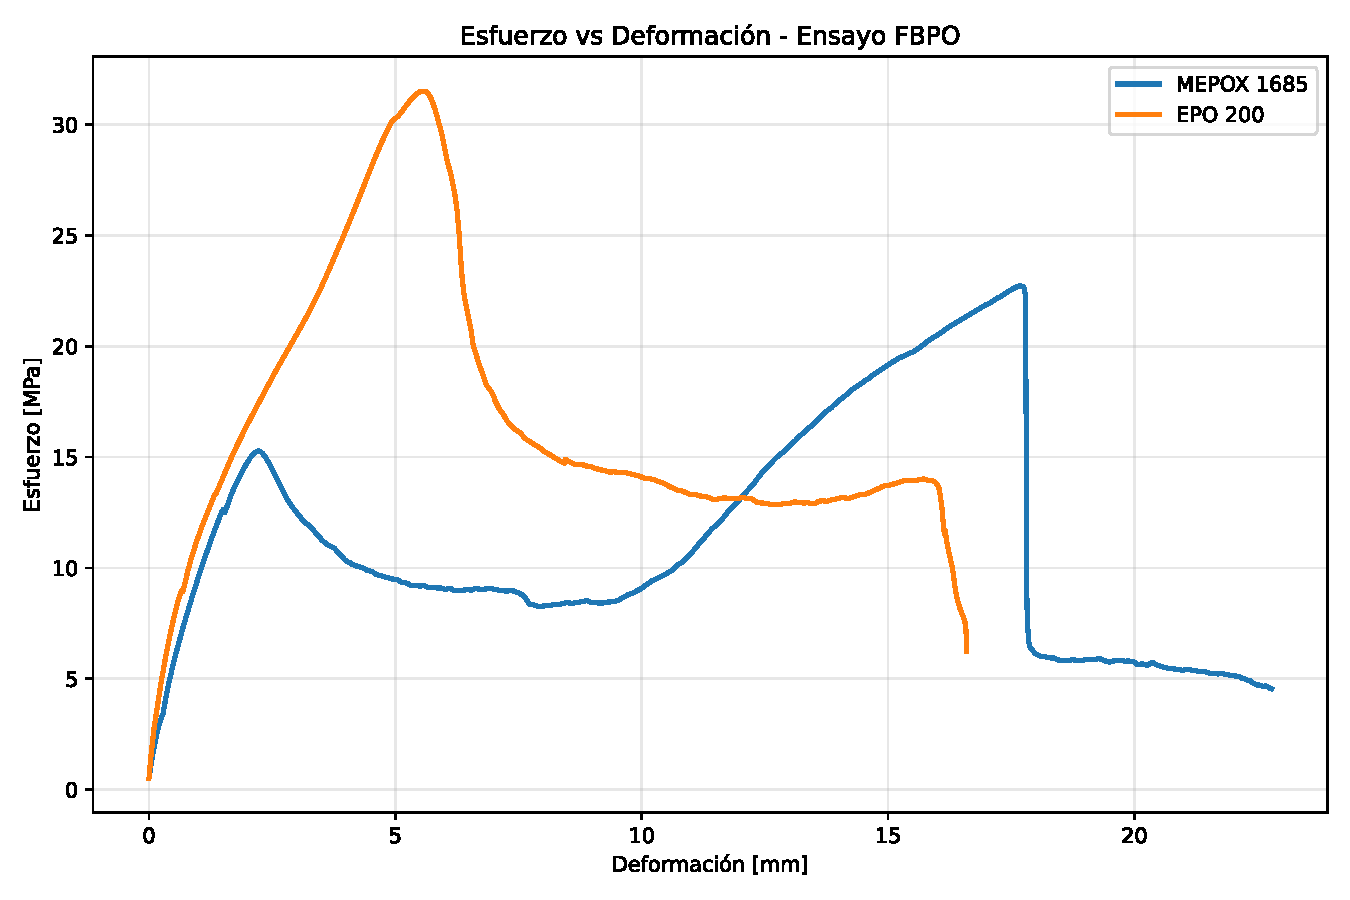
\includegraphics[width=0.85\textwidth]{Esf_v_def.pdf}
    \captionsetup{justification=centering, singlelinecheck=false}
    \caption{Curvas esfuerzo–desplazamiento representativas obtenidas durante los ensayos preliminares
    para los sistemas fibra–matriz evaluados.}
    \label{fig:esf_def_preliminar}
\end{figure}

\subsection{Resultados directos de las mediciones}

En esta subsección se presentan de manera conjunta los resultados directos obtenidos a partir de las
mediciones experimentales de IFSS aparente mediante el ensayo FBPO para los distintos sistemas
fibra–matriz evaluados. El análisis considera un total de 100 ensayos válidos, distribuidos en cuatro
grupos según el tipo de fibra y matriz: epo–HTA (40 ensayos), epo–HT (10 ensayos), mepox–HTA (40
ensayos) y mepox–HT (10 ensayos).

La \Cref{fig:IFSS_aparente} muestra el diagrama de caja correspondiente a los valores de IFSS aparente
obtenidos para cada sistema. En este gráfico se representan los valores individuales, la mediana, los
cuartiles y la dispersión asociada a cada conjunto de datos, permitiendo una visualización directa de
la variabilidad experimental y de las diferencias globales entre los sistemas analizados. De manera
general, se observa una dispersión distinta entre grupos y diferencias en los rangos de valores de
IFSS aparente, lo que sugiere comportamientos interfaciales diferenciados entre los sistemas
fibra–matriz considerados.

Los resultados aquí presentados tienen un carácter descriptivo y constituyen la base para el análisis
estadístico comparativo desarrollado en la subsección siguiente.

\begin{figure}[h!]
    \centering
    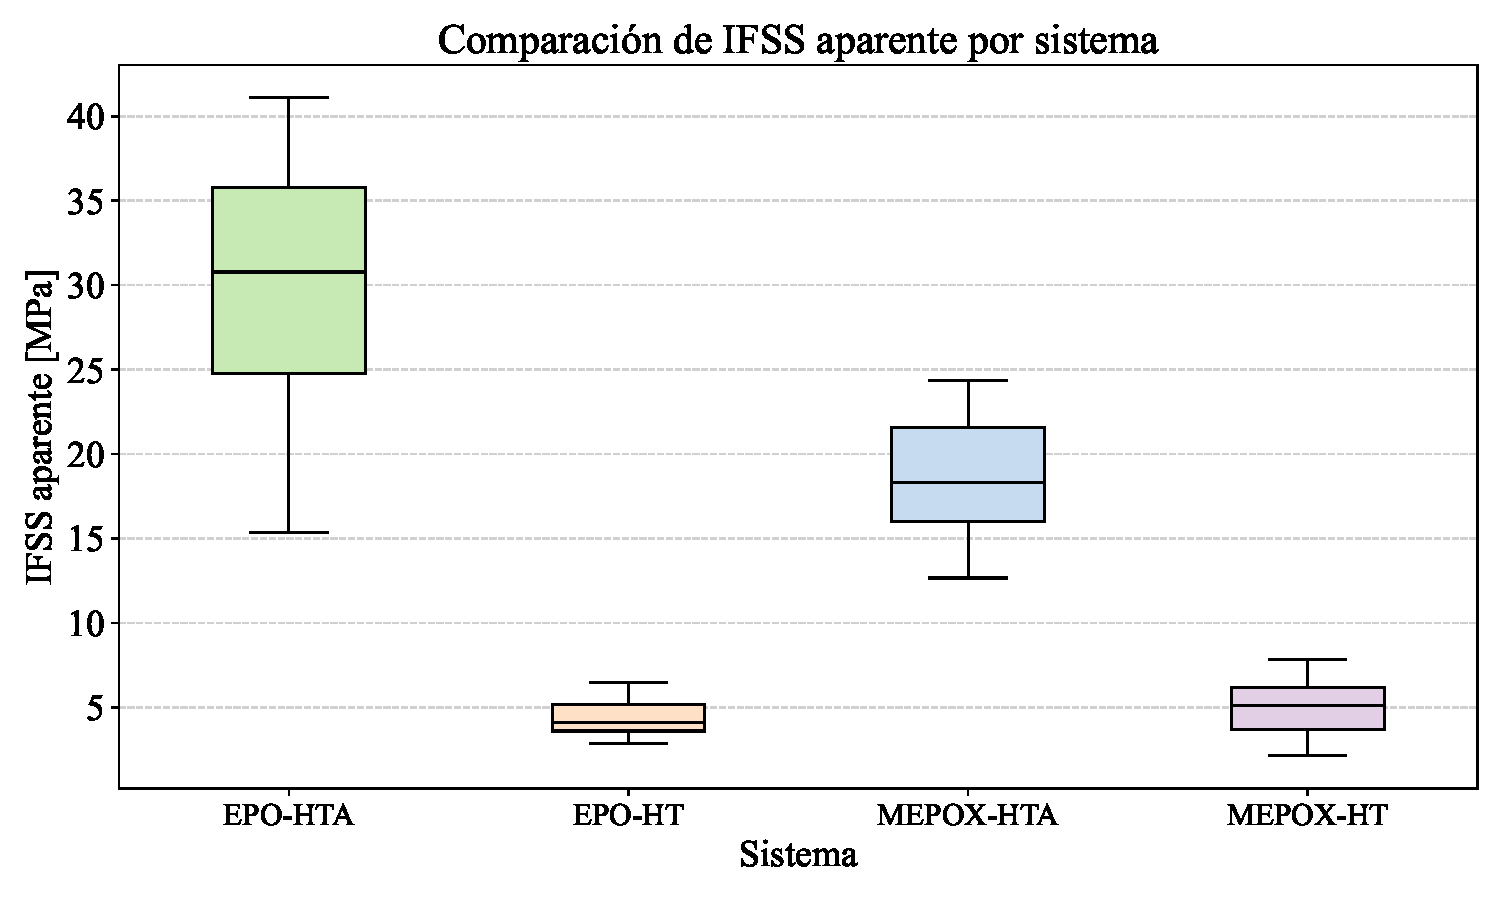
\includegraphics[width=0.85\textwidth]{IFSS_aparente.pdf}
    \captionsetup{justification=centering, singlelinecheck=false}
    \caption{Boxplot de los valores de IFSS aparente obtenidos para los sistemas evaluados.}
    \label{fig:IFSS_aparente}
\end{figure}

\subsection{Comparación con valores FBPO de referencia}

Con el objetivo de contextualizar los resultados experimentales obtenidos, se realizó una
comparación descriptiva entre los valores de IFSS aparente medidos en este trabajo y los rangos
típicos reportados en la literatura para ensayos de tipo Fiber-Bundle Pull-Out (FBPO).

La \Cref{fig:ifss_ranges} presenta, de manera comparativa, los rangos de IFSS recopilados a partir
de estudios previos junto con los valores experimentales obtenidos para los sistemas fibra–matriz
evaluados. Los rangos de referencia fueron sistematizados a partir de antecedentes bibliográficos
relevantes, permitiendo una visualización conjunta de la magnitud y dispersión de los valores
reportados para el método FBPO.

Esta comparación tiene un carácter estrictamente descriptivo y permite situar los resultados del
presente estudio dentro del contexto de valores típicamente reportados para el ensayo FBPO. En
este sentido, la figura proporciona un marco de referencia para la interpretación posterior de
los resultados y constituye un insumo para el análisis crítico desarrollado en la sección de
Discusión.

\begin{figure}[h!]
    \centering
    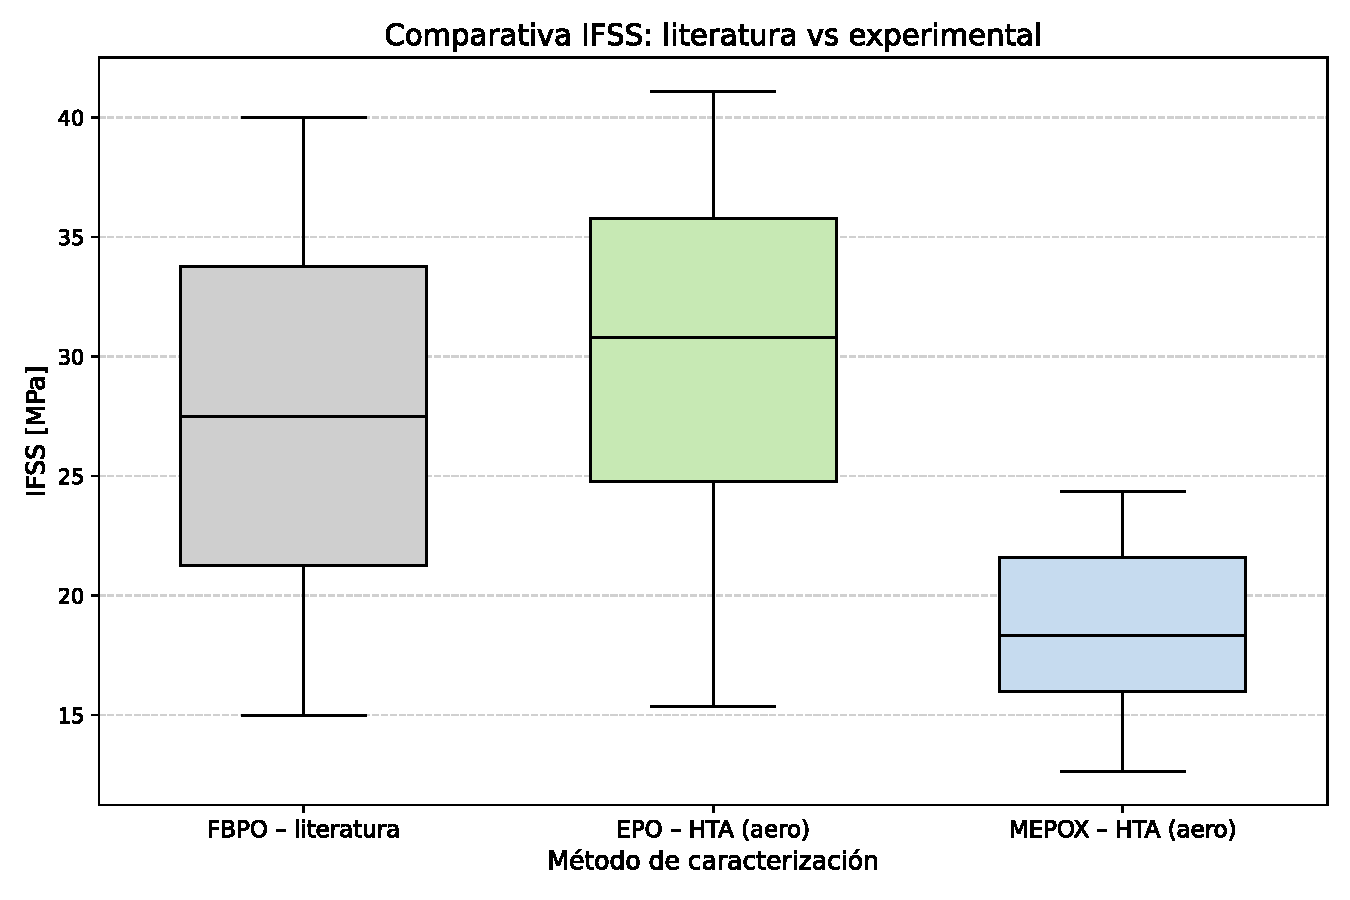
\includegraphics[width=0.75\textwidth]{Comparativa_Lit_Exp.pdf}
    \captionsetup{justification=centering, singlelinecheck=false}
    \caption{Comparación entre los valores de IFSS aparente obtenidos experimentalmente en este
    estudio y los rangos de IFSS reportados en la literatura para ensayos FBPO.}
    \label{fig:ifss_ranges}
\end{figure}

\subsection{Análisis estadístico de los resultados de IFSS aparente}

Con el propósito de evaluar la existencia de diferencias entre los sistemas fibra--matriz
analizados, se realizó un análisis estadístico sobre los valores de IFSS aparente obtenidos
experimentalmente.

Previo a la aplicación del análisis de varianza, se verificaron los supuestos estadísticos
correspondientes. La normalidad de los datos se evaluó mediante la prueba de Shapiro--Wilk,
no observándose desviaciones significativas en ninguno de los grupos analizados
($p > 0{,}05$). En contraste, la prueba de Levene evidenció heterogeneidad de varianzas entre
los grupos ($p \ll 0{,}05$), asociada a diferencias en la dispersión de los datos y al
desbalance en el número de probetas por sistema.

Dado que no se cumple el supuesto de homocedasticidad requerido para un ANOVA clásico, se
aplicó un análisis de varianza de Welch, el cual es robusto frente a varianzas desiguales y
tamaños muestrales desbalanceados. El resultado del ANOVA de Welch indicó la presencia de
diferencias significativas entre los sistemas evaluados.

\begin{table}[h!]
\centering
\caption{Resultados del análisis de varianza de Welch para los valores de IFSS aparente.}
\label{tab:anova_welch}
\begin{tabular}{lcccc}
\hline
Prueba & $F$ & gl$_1$ & gl$_2$ & $p$-valor \\
\hline
ANOVA de Welch & 279{,}54 & 3 & 36{,}46 & $< 0{,}001$ \\
\hline
\end{tabular}
\end{table}

Con el fin de identificar entre qué pares de sistemas se presentan diferencias significativas,
se realizó un análisis \emph{post hoc} mediante el método de Games--Howell, consistente con
el uso del ANOVA de Welch.

\begin{table}[h!]
\centering
\caption{Comparaciones múltiples mediante el método de Games--Howell.}
\label{tab:games_howell}
\begin{tabular}{l l c c c}
\hline
Grupo A & Grupo B & $\Delta$ media & $p$-valor & Significativo \\
\hline
epo--aero   & epo--fibra   & 25{,}52   & $< 0{,}001$ & Sí \\
epo--aero   & mepox--aero  & 11{,}27   & $< 0{,}001$ & Sí \\
epo--aero   & mepox--fibra & 24{,}96   & $< 0{,}001$ & Sí \\
epo--fibra  & mepox--aero  & $-14{,}25$ & $< 0{,}001$ & Sí \\
epo--fibra  & mepox--fibra & $-0{,}57$ & 0{,}85      & No \\
mepox--aero & mepox--fibra & 13{,}69   & $< 0{,}001$ & Sí \\
\hline
\end{tabular}
\end{table}

Los resultados del análisis estadístico confirman la existencia de diferencias entre los sistemas
fibra--matriz evaluados. La interpretación de estas diferencias y su relación con las
características de los materiales y del proceso se desarrollan en la sección de Discusión.